
\chapter{Introduction}
\label{ch:intro}
\section{Project Idea}
\begin{itemize}
\item Cortex is a research assistant over the user's own, live tools. The user asks a question in plain language, for example ``What changed in Orbit this week, and what's at risk?''. Instead of a single similarity search, Cortex runs a short, bounded pipeline: \emph{understand} (which sources are reachable now), \emph{recall} (what the user said matters), \emph{plan} (two to five sub-questions, each with its sources, keyword query and time window), \emph{search} (every sub-question against every chosen source, in parallel), \emph{synthesize} (a streamed answer that may use only numbered evidence and must cite it), \emph{verify} (each claim checked against what it cites), \emph{propose actions} (never execute) and \emph{remember} (only salient, durable facts).
\item The answer is presented as evidence rather than as prose to be trusted blindly. Each claim shows its verification state; unsupported claims are struck through; contradictions between sources (for example a Slack message and a GitHub milestone that give different dates) are listed as conflicts with both citations; and the full trace (plan, each tool call with its result count and latency, model calls) is available on demand.
\item The same pipeline feeds a proactive \emph{Daily Brief} (what changed in the last week and what is due in the next three, as cited cards), a \emph{Memory} inspector and a \emph{Connections} page for one-click OAuth through Composio.
\item A fictional sample workspace (a four-person student team building a campus events app, with deliberate cross-source conflicts) uses the same connector interface and actions as the live connectors, so the system can be demonstrated and evaluated without any personal accounts.
\end{itemize}


\section{Motivation of the Project}
\begin{itemize}
\item \textbf{Fragmented information costs time.} In the words of the McKinsey Global Institute, ``the average interaction worker spends an estimated 28 percent of the workweek managing e-mail and nearly 20 percent looking for internal information or tracking down colleagues who can help with specific tasks''~\cite{mckinseyweb}. Generative AI is expected to have its largest effect on exactly this kind of knowledge work~\cite{mckinsey}.
\item \textbf{Single-shot RAG is not analysis.} Multi-hop questions need several retrieval steps~\cite{trivedi2023ircot,press2023selfask}, and stuffing many retrieved chunks into a long context does not guarantee the model uses them: accuracy drops when relevant information sits in the middle of a long input~\cite{liu2024lost}. GRASP~\cite{grasp2026} shows that deciding \emph{how much} context to load is itself part of the problem.
\item \textbf{Trust needs evidence.} Language models produce fluent but unsupported statements. Citation benchmarks~\cite{gao2023alce} and fact-level scoring~\cite{min2023factscore} show that attribution can be measured; a product can therefore show the user which claims are supported instead of presenting everything with equal confidence.
\item \textbf{Agents that act must ask.} Once an agent can send e-mail or post messages, a wrong or injected instruction has real consequences. The Model Context Protocol makes tools easy to connect but also widens the attack surface~\cite{hou2025mcp}. A strict propose-then-approve design is a simple, verifiable safety property.
\item \textbf{Memory should be explainable.} Agent memory systems~\cite{packer2023memgpt,park2023generative} decide what to store on the user's behalf. Users should be able to see why something was remembered, where it came from, how long it will be kept, and remove it.
\item \textbf{Cost.} Students and individual developers cannot pay per-token API prices; a design that stays within free tiers makes the system usable by its intended users.
\end{itemize}

\section{Literature Survey}
\begin{itemize}
\item \textbf{Retrieval-augmented generation.} Lewis et al.~\cite{lewis2020rag} combine a parametric seq2seq generator with a non-parametric dense index. In the RAG-Sequence model the output probability marginalises over the top-$k$ retrieved passages $z$:
\[ p(y \mid x) \approx \sum_{z \in \mathrm{top}\mbox{-}k(p_\eta(\cdot \mid x))} p_\eta(z \mid x) \prod_{i} p_\theta(y_i \mid x, z, y_{1:i-1}). \]
The retriever is queried once per input. Cortex keeps the conditioning on retrieved evidence but replaces the single dense index with several live tools that are searched through their own APIs, and it exposes the retrieved passages as numbered, citable evidence.

\item \textbf{Agentic and multi-step retrieval.} ReAct~\cite{yao2023react} lets the model alternate a \emph{thought} with an \emph{action} (for example a Wikipedia search) and the resulting \emph{observation}, producing a trajectory $(t_1, a_1, o_1, \ldots, t_n, a_n, o_n)$ that reduces hallucination on HotpotQA and FEVER. IRCoT~\cite{trivedi2023ircot} interleaves retrieval with each chain-of-thought sentence, using the sentence generated so far as the next query. Self-Ask~\cite{press2023selfask} defines the \emph{compositionality gap}, the rate at which a model answers all sub-questions correctly but the composed question wrongly, and narrows it by asking explicit follow-up questions. Singh et al.~\cite{singh2025agenticrag} survey these designs as \emph{agentic RAG}: retrieval controlled by agents that plan, reflect, use tools and collaborate. Cortex is a planning-based agentic RAG system: the plan is produced once, then executed in parallel.

\item \textbf{Base paper: GRASP.} Gandhi, Lee et al.~\cite{grasp2026} argue that an agentic RAG system faces three linked decisions: when to search, which kind of matching to use (exact terms or meaning), and how much text to bring into the context, since extra, irrelevant text can mislead the agent. GRASP gives the agent three actions (semantic search, keyword search, and reading a paragraph around a retrieved sentence) and trains the policy with reinforcement learning. The reward combines answer accuracy, grounded reading, complementary use of the search tools and turn efficiency. On HotpotQA, 2WikiMultiHopQA and MuSiQue (500 validation questions each) the authors report retrieval recall of 0.90, 0.90 and 0.70 and higher answer scores than all of their baselines, which include one-shot retrieval, prompted agents and other agents trained with reinforcement learning. In the authors' analysis, the trained agent first searches by meaning to find the right topic, then reads a paragraph to confirm the details, and finally searches by keyword for the specific entity it has found, a pattern they liken to skimming and scanning. Cortex does not train a policy; it transfers three of these lessons to a prompting-based system over live tools: (i) retrieve small, citable units (each evidence item is a quote of at most a few hundred characters with title, author, timestamp and link) and keep at most 16 of them; (ii) use keyword queries, because the tool APIs it calls (Gmail, Slack, GitHub search) are lexical, while long-term memory search can be semantic when Oracle Agent Memory is configured; and (iii) bound the number of retrieval turns explicitly, with a single broadened retry for sub-questions that found nothing.

\item \textbf{Adaptive and corrective retrieval.} Self-RAG~\cite{asai2024selfrag} trains one model that retrieves on demand and emits reflection tokens judging whether a passage is relevant and whether its own output is supported. Corrective RAG (CRAG)~\cite{yan2024crag} adds a light-weight evaluator that scores retrieved documents and, depending on the score, uses them, searches the web, or both, followed by a decompose-then-recompose filter. Adaptive-RAG~\cite{jeong2024adaptiverag} trains a small classifier to predict question complexity and selects no retrieval, single-step or multi-step retrieval accordingly. Search-R1~\cite{jin2025searchr1} trains a model with reinforcement learning to issue search queries during step-by-step reasoning. These approaches need model training or fine-tuning; Cortex obtains a coarse version of the same adaptivity without training, through the user-selected Fast and Deep modes, the planner's \emph{chat} intent (no retrieval for small talk), and the empty-result retry.

\item \textbf{Attribution and verification.} ALCE~\cite{gao2023alce} evaluates generation with citations along fluency, correctness and citation quality; citation recall asks whether each statement is fully supported by the passages it cites, and citation precision whether each citation is needed. RARR~\cite{gao2023rarr} finds attribution for model output with search and post-edits unsupported content. FActScore~\cite{min2023factscore} splits text into atomic facts and computes
\[ f(y) = \frac{1}{|A_y|} \sum_{a \in A_y} \mathbb{I}[a \mbox{ is supported by } \mathcal{C}], \]
the fraction of atomic facts supported by a knowledge source $\mathcal{C}$. RAGAS~\cite{es2024ragas} proposes reference-free metrics for RAG pipelines, including faithfulness of the answer to the retrieved context. Cortex's groundedness score is a sentence-level, citation-scoped variant of these ideas, computed cheaply (lexically) for every claim, with a model-based re-check only for doubtful claims.

\item \textbf{Long-term memory for agents.} MemGPT~\cite{packer2023memgpt} manages a model's limited context like an operating system manages memory, moving information between the context window and external storage. Generative Agents~\cite{park2023generative} store a stream of observations and retrieve memories by a weighted sum of recency, importance and relevance. Cortex's memory service uses the same three signals (salience as importance, exponential decay as recency, search score as relevance) but makes them visible to the user, keeps a reason and a source for each memory, and lets the user pin, edit or forget it.

\item \textbf{Tool use and the Model Context Protocol.} Toolformer~\cite{schick2023toolformer} shows that a model can learn in a self-supervised way which external APIs to call and with which arguments. The Model Context Protocol (MCP)~\cite{anthropic2024mcp} standardises how assistants connect to tools and data; Hou et al.~\cite{hou2025mcp} survey its ecosystem and its security threats across the server life cycle. Cortex uses MCP both through Composio's hosted endpoint and for arbitrary servers declared in a configuration file, and it treats every write operation as a proposal that needs explicit approval.

\item \textbf{Long contexts.} Liu et al.~\cite{liu2024lost} show that models use information at the beginning and end of a long input much better than information in the middle. This supports keeping the evidence set small and ranked, as GRASP's granularity argument also suggests.
\end{itemize}

Table~\ref{tab:litcompare} compares the closest approaches with Cortex on the properties this project targets.

\begin{table}[!htbp]
\begin{center}
\def\arraystretch{1.3}
\small
\begin{tabularx}{\textwidth}{| X | c | c | c | c | c |}
\hline
Approach & Multi-step & Training-free & Claim check & Live tools & Consent gate \\ \hline
RAG~\cite{lewis2020rag} & No & No & No & No & -- \\ \hline
ReAct~\cite{yao2023react} & Yes & Yes & No & Yes & No \\ \hline
IRCoT~\cite{trivedi2023ircot} & Yes & Yes & No & No & -- \\ \hline
Self-RAG~\cite{asai2024selfrag} & Yes & No & Self-critique & No & -- \\ \hline
CRAG~\cite{yan2024crag} & Partly & No & Retrieval check & Web & -- \\ \hline
Adaptive-RAG~\cite{jeong2024adaptiverag} & Adaptive & No & No & No & -- \\ \hline
GRASP~\cite{grasp2026} & Yes & No (RL) & Grounded-reading reward & No & -- \\ \hline
Cortex (this work) & Yes (bounded) & Yes & Per claim & Yes & Yes \\ \hline
\end{tabularx}
\end{center}
\caption{Comparison of related approaches with Cortex}
\label{tab:litcompare}
\end{table}


\chapter{Problem Definition and scope}
\section{Problem Statement}
Given a question $q$ from a user whose work data lives in several independently hosted tools, produce, within a bounded number of model calls and tool calls, an answer that (a) uses only evidence retrieved from those tools during the run, (b) cites the evidence for every factual sentence, (c) reports how much of the answer is supported, (d) reports where the sources disagree and what could not be found, and (e) turns any requested write operation into a proposal that the user must approve before it runs. The system must keep working when individual sources or model providers fail, and it must remember only what is likely to matter later, in a way the user can inspect and control.


\subsection{Goals and objectives}
Goal and Objectives:
\begin{itemize}
  	\item \textbf{Overall goal:} a trustworthy, free-to-run research assistant over live work data.
  	\item \textbf{Input (ask):} an HTTP \texttt{POST /api/ask} request with a JSON body \texttt{\{question, mode, threadId?, history?\}}. \texttt{question} is a non-empty string of at most 2000 characters; \texttt{mode} is \texttt{"fast"} or \texttt{"deep"} (any other value is treated as \texttt{"deep"}); \texttt{history} is the recent conversation, of which the last six turns are used, each cut to 1500 characters. The user identity is an anonymous per-browser identifier held in an HTTP-only cookie.
  	\item \textbf{Output (ask):} a \texttt{text/event-stream} response. Each event is one JSON object of a fixed type: \texttt{run}, \texttt{step} (seven steps, each \texttt{active}, \texttt{done} or \texttt{skipped}, with its duration), \texttt{memory\_used}, \texttt{plan}, \texttt{tool\_call}, \texttt{tool\_result}, \texttt{evidence}, \texttt{source\_error}, \texttt{token}, \texttt{answer}, \texttt{verdict} (claims, groundedness, conflicts, missing items, follow-up questions), \texttt{action\_proposal}, \texttt{memory\_written}, \texttt{usage}, \texttt{error} and \texttt{done}.
  	\item \textbf{Input/output (approve):} \texttt{POST /api/actions/\{id\}} with \texttt{\{decision: "approve" | "reject", edits?\}} returns the updated proposal with status \texttt{executed}, \texttt{failed} or \texttt{rejected}; a second decision on the same proposal is refused with HTTP 409.
  	\item \textbf{Other outputs:} the Daily Brief (\texttt{GET /api/brief}), the memory list and its pin, edit and forget operations (\texttt{/api/memory}), and the connection list and OAuth start (\texttt{/api/connections}).
\end{itemize}

 \subsection{Statement of scope}
	\begin{itemize}
	\item	\textbf{Size and bounds of input:} question length $\le 2000$ characters (longer questions are rejected with a message); history $\le 6$ turns; plan $\le 5$ sub-questions; search calls $\le 18$ per run; each connector returns at most 6 items per call (4 in Fast mode); at most 16 evidence items (8 in Fast mode) reach the model; at most 3 action proposals and 2 memory writes per run. \textbf{Input validation:} an empty question is rejected; planner output is validated against a schema and replaced by a local single-step plan if unusable; action proposals are validated against the connector's declared actions and required parameters; memory writes are validated for length (3--500 characters) and salience in $[0,1]$. \textbf{Input dependency:} the plan depends on the connected sources and on recalled memories; the answer depends on the evidence; verification depends on the answer and the evidence. The I/O state behaviour of an action is shown in Figure~\ref{fig:state-dig}.
	\item \textbf{What the product is:} a web application and a set of reusable packages (agent, connectors, model router) plus a memory service, which answer questions over connected tools with cited, verified answers, propose actions, and keep an explainable memory. \textbf{What it is not:} it is not a search index or a data warehouse (it does not copy users' data; it queries the tools at question time and caches results for 90~s), it does not train or fine-tune models, it does not execute any write operation on its own, and it does not yet implement the time-travel (snapshot diff) queries, the editable plan, or the Cortex-as-an-MCP-server interface described in the project vision; those are future work.
	\end{itemize}


\section{Major Constraints}
\begin{itemize}
\item \textbf{Free-tier quotas.} All language models are used through free tiers with per-minute and per-day limits that change often. This constrains the number of model calls per question (at most 4 in Deep mode, 2 in Fast mode), requires failover across providers with cooldowns, and motivates the response cache.
\item \textbf{Third-party APIs.} Connectors depend on Composio, the MCP servers and Firecrawl; tool names and output shapes can change. Tool identifiers are therefore stored as data, and tool output is mapped to evidence by a tolerant extractor.
\item \textbf{Privacy and consent.} The system reads private mail and chat. It must not store users' source data beyond short-lived caches, must not expose OAuth tokens to the browser, and must not perform write operations without explicit approval.
\item \textbf{Latency.} An interactive answer should start within a few seconds. Searches run in parallel with a 12~s timeout per call, and the answer is streamed.
\item \textbf{Memory backend.} Oracle Agent Memory provides only a Python SDK, which forces a separate Python service. The Oracle AI Database container could not be used at the time of writing because of a Docker networking issue, so the SQLite fallback is the active backend.
\item \textbf{Team and time.} A four-member team within one academic year, alongside regular coursework.
\end{itemize}

\section{Methodologies of Problem solving and efficiency issues}
\begin{itemize}
	\item The problem can be solved in several ways. Table~\ref{tab:approaches} compares them on the number of model calls per question, which dominates both latency and free-tier cost, and on other efficiency and quality issues.
\end{itemize}

\begin{table}[!htbp]
\begin{center}
\def\arraystretch{1.3}
\small
\begin{tabularx}{\textwidth}{| p{3.2cm} | c | X |}
\hline
Approach & Model calls & Efficiency and quality issues \\ \hline
Single-shot RAG over a copied index & 1 & Needs ingesting and re-indexing every tool; stale data; one retrieval round misses multi-hop evidence; no claim check. \\ \hline
Unbounded ReAct loop & $n$ (unbounded) & Calls grow with the number of steps; hard to keep within free quotas; latency varies widely; can loop. \\ \hline
RL-trained search policy (GRASP, Search-R1) & several per question & Best retrieval decisions, but requires training data, GPUs and a model the team can fine-tune; not feasible with hosted free-tier APIs. \\ \hline
Graph framework with human interrupts & varies & Flexible, but adds a framework dependency and makes the call count less predictable. \\ \hline
\textbf{Bounded plan-then-execute pipeline (chosen)} & Deep $\le 4$, Fast $\le 2$ & One planning call, parallel searches (no model call), one streamed synthesis, an optional verification call for doubtful claims only. ``Not found'' answers use no model call. Predictable cost and latency. \\ \hline
\end{tabularx}
\end{center}
\caption{Alternative methodologies and their efficiency}
\label{tab:approaches}
\end{table}

Further efficiency measures in the chosen design: identical prompts are served from a least-recently-used cache (default lifetime 6~h, persisted to disk); identical searches within 90~s are served from a search cache; the planner and the verifier use the faster model tier and only the synthesis uses the stronger tier; and the lexical verifier, which is linear in the number of claim and evidence tokens, runs before any model-based check.

\section{Outcome}
\begin{itemize}
\item A working web application (Ask with live trace, Brief, Memory, Connections) and an agent API that answers questions over six work tools and the web with cited, verified answers.
\item Reusable packages: a free-tier model router with failover, cooldowns and caching; a connector registry with Composio, generic MCP, Firecrawl and sample-workspace connectors; and a memory service with provenance, decay and governance.
\item A consent model in which only one endpoint can execute an action, once, for the user who received the proposal, within 30 minutes.
\item An automated test suite (18 tests) and an evaluation harness with preliminary results (mean groundedness 0.88, citation recall 0.92, zero actions executed without consent).
\end{itemize}

\section{Applications}
\begin{itemize}
\item Students and project teams: tracking deadlines, advisor requests and blockers across e-mail, chat, documents and repositories.
\item Software developers: status of issues and pull requests, review requests and release dates across GitHub, Slack and documentation.
\item Professionals: a morning brief of what changed and what is at risk, ranked by remembered priorities.
\item Any organisation that wants answers over internal tools with an auditable link from each claim to its source, and with human approval before an assistant sends or changes anything.
\end{itemize}

\section{Hardware Resources Required}
\begin{table}[!htbp]
\begin{center}
\def\arraystretch{1.5}
  \begin{tabular}{| c | c | c | p{6cm} |}
\hline
Sr. No. &	Parameter &	Minimum Requirement & Justification \\
\hline
1 &	CPU Speed &	 2 GHz, dual core  & Runs the Next.js server, the Python memory service and the browser at the same time; model inference happens at the providers. \\
\hline
2 &	RAM  &	8 GB &  The Next.js development server, Node.js, the Python service and a browser together need several gigabytes; the optional Oracle Database Free container needs more. \\
 \hline
3 & Storage & 5 GB free & Node.js dependencies, the Python virtual environment, caches and the SQLite ledger. \\
\hline
4 & Network & Broadband Internet & Every model call and live connector call is a remote API request. \\
\hline
\end{tabular}
 \caption { Hardware Requirements }
 \label{tab:hreq}
\end{center}

\end{table}


\section{Software Resources Required}
Platform :
\begin{enumerate}
\item Operating System: Windows 10/11, Linux or macOS (development was done on Windows 11).
\item IDE: Visual Studio Code.
\item Programming Language: TypeScript on Node.js 24 or later (web application, agent, connectors, router); Python 3.11 (memory service).
\item Frameworks and libraries: Next.js 16 with React 19 and Tailwind CSS 4; Zod; the OpenAI-compatible client library; the Composio SDK; the MCP TypeScript SDK; the Firecrawl SDK; the LangSmith SDK; FastAPI, Uvicorn and Pydantic; \texttt{oracledb} and \texttt{oracleagentmemory} (optional); Vitest.
\item External services (free tiers): Groq, Google Gemini, Cerebras, OpenRouter and Puter (model providers); Composio; Firecrawl; LangSmith; Oracle AI Database (optional).
\end{enumerate}




\chapter{Project Plan}

\section{Project Estimates}
The project follows the waterfall model: requirement analysis, feasibility study, design, implementation, testing and maintenance, each completed and reviewed before the next. The estimates below use the basic COCOMO model together with the outputs of the laboratory assignments in Annexures~\ref{app:algo} and~\ref{app:quality}.
\subsection{Reconciled Estimates}
\subsubsection{Cost Estimate}
The size of the delivered source code, counted as non-blank lines of TypeScript, TSX, Python, CSS and scripts (excluding dependencies and generated files), is about 6.1~KLOC. The basic COCOMO model for an organic project gives
\[ E = 2.4 \times (\mathrm{KLOC})^{1.05} = 2.4 \times 6.1^{1.05} \approx 16.0 \mbox{ person-months}. \]
The monetary cost of operation is zero: every external service is used on its free tier (Table~\ref{tab:cost}). The only expenses are the team's own computers and Internet connection. If a notional labour rate is needed for comparison, the effort can be multiplied by a rate chosen by the department; no such rate is assumed here.

\begin{table}[!htbp]
\begin{center}
\def\arraystretch{1.3}
\begin{tabular}{| l | l | c |}
\hline
Resource & Plan used & Cost (INR) \\ \hline
Language models (Groq, Gemini, Cerebras, OpenRouter) & Free tier & 0 \\ \hline
Puter (last-resort model fallback) & User-pays free credit & 0 \\ \hline
Composio (managed OAuth connectors) & Free plan & 0 \\ \hline
Firecrawl (web evidence) & Free plan & 0 \\ \hline
LangSmith (tracing) & Developer (free) plan & 0 \\ \hline
Oracle AI Database & Free container / Always Free & 0 \\ \hline
Development tools (VS Code, Node.js, Python, Git) & Open source / free & 0 \\ \hline
\end{tabular}
\end{center}
\caption{Operating cost of the project}
\label{tab:cost}
\end{table}

\subsubsection{Time Estimates}
The development time from basic COCOMO is
\[ D = 2.5 \times E^{0.38} = 2.5 \times 16.0^{0.38} \approx 7.2 \mbox{ months}, \]
with an average staffing of $E/D \approx 2.2$ persons. With four team members working part-time alongside coursework, this fits the academic year (about ten months including documentation and evaluation). The phase-wise schedule is in Section~\ref{sec:schedule} and Annexure~\ref{app:plan}.


\subsection{Project Resources}
\begin{itemize}
\item \textbf{People:} four students (see Section~\ref{sec:team}) and the internal guide.
\item \textbf{Hardware:} the team's laptops (Table~\ref{tab:hreq}); no dedicated server is needed for development.
\item \textbf{Software and tools:} as listed in the software resources section; Git for version control.
\item \textbf{Memory sharing, IPC and concurrency:} the web server and the memory service are separate processes that communicate over HTTP/JSON on the local machine; the agent and the browser communicate over a server-sent event stream; within the server, search calls run concurrently as asynchronous promises; the memory service serialises access to its SQLite database with a lock; and the process-wide singletons (model router, action store, connector registries) are shared by all requests in one Node.js process.
\end{itemize}

\section{Risk Management w.r.t. NP Hard analysis}
This section discusses Project risks and the approach to managing them.
\subsection{Risk Identification}
For risks identification, review of scope document, requirements specifications and schedule is done. Answers to questionnaire revealed some risks. Each risk is categorized as per the categories mentioned in \cite{bookPressman}. Please refer table \ref{tab:risk} for all the risks. The questions below are quoted from the risk identification questionnaire in Pressman and Maxim~\cite{bookPressman}; the team's answers are given after each question.

\begin{enumerate}
\item Have top software and customer managers formally committed to support the project? \emph{Yes; it is an internal project approved by the department, with no external customer.}
\item Are end-users enthusiastically committed to the project and the system/product to be built? \emph{Not yet established; there are no real users yet, so the sample workspace and the evaluation stand in for user feedback.}
\item Are requirements fully understood by the software engineering team and its customers? \emph{Mostly; the core requirements are fixed, while some vision items (time-travel queries, editable plan) are deferred.}
\item Have customers been involved fully in the definition of requirements? \emph{No external customer; requirements come from the team and the guide.}
\item Do end-users have realistic expectations? \emph{The interface states uncertainty explicitly (struck-through claims, ``not found'' answers) to keep expectations realistic.}
\item Does the software engineering team have the right mix of skills? \emph{Partly; agent design, web development and Python are covered, while database operations (Oracle) were new.}
\item Are project requirements stable? \emph{The functional requirements are stable; external APIs and free-tier limits are not.}
\item Is the number of people on the project team adequate to do the job? \emph{Yes for the current scope (Section~\ref{sec:team}).}
\item Do all customer/user constituencies agree on the importance of the project and on the requirements for the system/product to be built? \emph{Yes within the team and with the guide.}
\end{enumerate}

\subsection{Risk Analysis}
The risks for the Project can be analyzed within the constraints of time and quality

\begin{table}[!htbp]
\begin{center}
%\def\arraystretch{1.5}
\def\arraystretch{1.5}
\begin{tabularx}{\textwidth}{| c | X | c | c | c | c |}
\hline
\multirow{2}{*}{ID} & \multirow{2}{*}{Risk Description}	& \multirow{2}{*}{Probability} & \multicolumn{3}{|c|}{Impact} \\ \cline{4-6}
	& & &	Schedule	& Quality	& Overall \\ \hline
1	& Free-tier model limits, quota changes or model removals stop answers	& High	& Medium	& High	& High \\ \hline
2	& Connector APIs (Composio tool names, MCP servers) change or fail	& Medium	& Medium	& High	& High \\ \hline
3	& Answers contain unsupported or hallucinated claims	& Medium	& Low	& Very High	& High \\ \hline
4	& The agent performs an unintended action (e.g. after prompt injection)	& Low	& Low	& Very High	& Very High \\ \hline
5	& The Oracle memory backend cannot be brought up	& High	& Medium	& Medium	& Medium \\ \hline
6	& Private user data is exposed or retained	& Low	& Low	& Very High	& High \\ \hline
\end{tabularx}
\end{center}
\caption{Risk Table}
\label{tab:risk}
\end{table}


\begin{table}[!htbp]
\begin{center}
%\def\arraystretch{1.5}
\def\arraystretch{1.5}
\begin{tabular}{| c | c | c |}
\hline
Probability & Value &	Description \\ \hline
High &	Probability of occurrence is &  $ > 75 \% $ \\ \hline
Medium &	Probability of occurrence is  & $26-75 \% $ \\ \hline
Low	& Probability of occurrence is & $ < 25 \% $ \\ \hline
\end{tabular}
\end{center}
\caption{Risk Probability definitions \cite{bookPressman}}
\label{tab:riskdef}
\end{table}

\begin{table}[!htbp]
\begin{center}
%\def\arraystretch{1.5}
\def\arraystretch{1.5}
\begin{tabularx}{\textwidth}{| c | c | X |}
\hline
Impact & Value	& Description \\ \hline
Very high &	$> 10 \%$ & Schedule impact or Unacceptable quality \\ \hline
High &	$5-10 \%$ & Schedule impact or Some parts of the project have low quality \\ \hline
Medium	& $ < 5 \% $ & Schedule impact or Barely noticeable degradation in quality Low	Impact on schedule or Quality can be incorporated \\ \hline
\end{tabularx}
\end{center}
\caption{Risk Impact definitions \cite{bookPressman}}
\label{tab:riskImpactDef}
\end{table}

\subsection{Overview of Risk Mitigation, Monitoring, Management}


Following are the details for each risk.
\begin{table}[!htbp]
\begin{center}
%\def\arraystretch{1.5}
\def\arraystretch{1.5}
\begin{tabularx}{\textwidth}{| l | X |}
\hline
Risk ID	& 1 \\ \hline
Risk Description	& Free-tier model limits, quota changes or model removals stop answers. \\ \hline
Category	& Technology \\ \hline
Source	& Live testing with real keys (rate-limit and ``model not found'' responses). \\ \hline
Probability	& High \\ \hline
Impact	& High \\ \hline
Response	& Mitigate \\ \hline
Strategy	& Failover router across several providers; cooldowns per error type (rate limit, invalid key, out of credit, model not found); one wait of up to 12~s for the soonest provider; response cache; model identifiers configurable through environment variables; Fast Mode as a one-call fallback. \\ \hline
Risk Status	& Occurred; mitigated \\ \hline
\end{tabularx}
\end{center}
%\caption{Risk Impact definitions \cite{bookPressman}}
\label{tab:risk1}
\end{table}

\begin{table}[!htbp]
\begin{center}
%\def\arraystretch{1.5}
\def\arraystretch{1.5}
\begin{tabularx}{\textwidth}{| l | X |}
\hline
Risk ID	& 2 \\ \hline
Risk Description	& Connector APIs change or fail. \\ \hline
Category	& Technology / External dependency \\ \hline
Source	& Software Design Specification documentation review. \\ \hline
Probability	& Medium \\ \hline
Impact	& High \\ \hline
Response	& Mitigate \\ \hline
Strategy	& Tool identifiers kept as data in one file; tolerant evidence extraction from any output shape; per-call timeout, one retry and a short cache; a failed source is reported with its impact while the run continues; a service check script verifies every configured tool. \\ \hline
Risk Status	& Identified; mitigated \\ \hline
\end{tabularx}
\end{center}
\label{tab:risk2}
\end{table}

\begin{table}[!htbp]
\begin{center}
%\def\arraystretch{1.5}
\def\arraystretch{1.5}
\begin{tabularx}{\textwidth}{| l | X |}
\hline
Risk ID	& 3 \\ \hline
Risk Description	& Answers contain unsupported or hallucinated claims. \\ \hline
Category	& Product quality \\ \hline
Source	& Literature survey and early testing. \\ \hline
Probability	& Medium \\ \hline
Impact	& Very High \\ \hline
Response	& Mitigate \\ \hline
Strategy	& Evidence-only prompt that requires a citation per factual sentence; lexical claim verification with a model re-check for doubtful claims; struck-through unsupported claims and a groundedness score in the interface; ``not found'' answered without a model call; groundedness measured by the evaluation harness. \\ \hline
Risk Status	& Identified; monitored by evaluation \\ \hline
\end{tabularx}
\end{center}
\label{tab:risk3}
\end{table}

\begin{table}[!htbp]
\begin{center}
\def\arraystretch{1.5}
\begin{tabularx}{\textwidth}{| l | X |}
\hline
Risk ID	& 4 \\ \hline
Risk Description	& The agent performs an unintended action. \\ \hline
Category	& Security \\ \hline
Source	& Threat review of tool use and MCP~\cite{hou2025mcp}. \\ \hline
Probability	& Low \\ \hline
Impact	& Very High \\ \hline
Response	& Avoid \\ \hline
Strategy	& The agent can only propose; proposals are validated, stored server-side and shown with an exact preview; one endpoint executes an approved proposal once, for the same user, within 30 minutes; tests and the evaluation check that nothing runs without consent. \\ \hline
Risk Status	& Identified; controlled (0 unconsented executions measured) \\ \hline
\end{tabularx}
\end{center}
\label{tab:risk4}
\end{table}

\begin{table}[!htbp]
\begin{center}
\def\arraystretch{1.5}
\begin{tabularx}{\textwidth}{| l | X |}
\hline
Risk ID	& 5 \\ \hline
Risk Description	& The Oracle memory backend cannot be brought up. \\ \hline
Category	& Development Environment \\ \hline
Source	& Setting up the local Oracle AI Database Free container. \\ \hline
Probability	& High \\ \hline
Impact	& Medium \\ \hline
Response	& Mitigate \\ \hline
Strategy	& The memory service offers the same API on SQLite with full-text search and reports the active backend on its health endpoint; Oracle remains optional. \\ \hline
Risk Status	& Occurred (Docker networking issue); fallback in use \\ \hline
\end{tabularx}
\end{center}
\label{tab:risk5}
\end{table}

\begin{table}[!htbp]
\begin{center}
\def\arraystretch{1.5}
\begin{tabularx}{\textwidth}{| l | X |}
\hline
Risk ID	& 6 \\ \hline
Risk Description	& Private user data is exposed or retained. \\ \hline
Category	& Security / Privacy \\ \hline
Source	& Requirements review. \\ \hline
Probability	& Low \\ \hline
Impact	& Very High \\ \hline
Response	& Mitigate \\ \hline
Strategy	& Managed OAuth so the browser never sees tokens; no copying of source data into a store (only 90~s search caches); only selected memories are kept, each with an expiry and a forget control; memories of the sample workspace are kept apart from real ones. \\ \hline
Risk Status	& Identified \\ \hline
\end{tabularx}
\end{center}
\label{tab:risk6}
\end{table}

\section{Project Schedule}
\label{sec:schedule}
\subsection{Project task set}
\label{sec:taskset}
Major Tasks in the Project stages are:
\begin{itemize}
  \item Task 1: Problem identification, literature survey (base paper GRASP and related work) and requirement gathering.
  \item Task 2: Software requirement specification, feasibility study and risk analysis.
  \item Task 3: Architecture and detailed design (agent pipeline, connectors, router, memory, interfaces).
  \item Task 4: Feasibility spikes: free-tier model failover, Composio OAuth and tools, Oracle Agent Memory.
  \item Task 5: Implementation of the core: model router, connector registry and connectors, agent pipeline, action store, memory service.
  \item Task 6: Implementation of the web application: Ask with live trace, Brief, Memory, Connections.
  \item Task 7: Testing and evaluation: unit and integration tests, evaluation harness, live service checks.
  \item Task 8: Term-I report and paper preparation.
  \item Task 9: Term-II work: Oracle memory backend, larger evaluation set, deployment.
  \item Task 10: Final report, demonstration and submission.
\end{itemize}

\subsection{Task network}
Project tasks and their dependencies are noted in this diagrammatic form (Figure~\ref{fig:tasknet}).

\begin{figure}[!htbp]
\centering
\resizebox{\textwidth}{!}{%
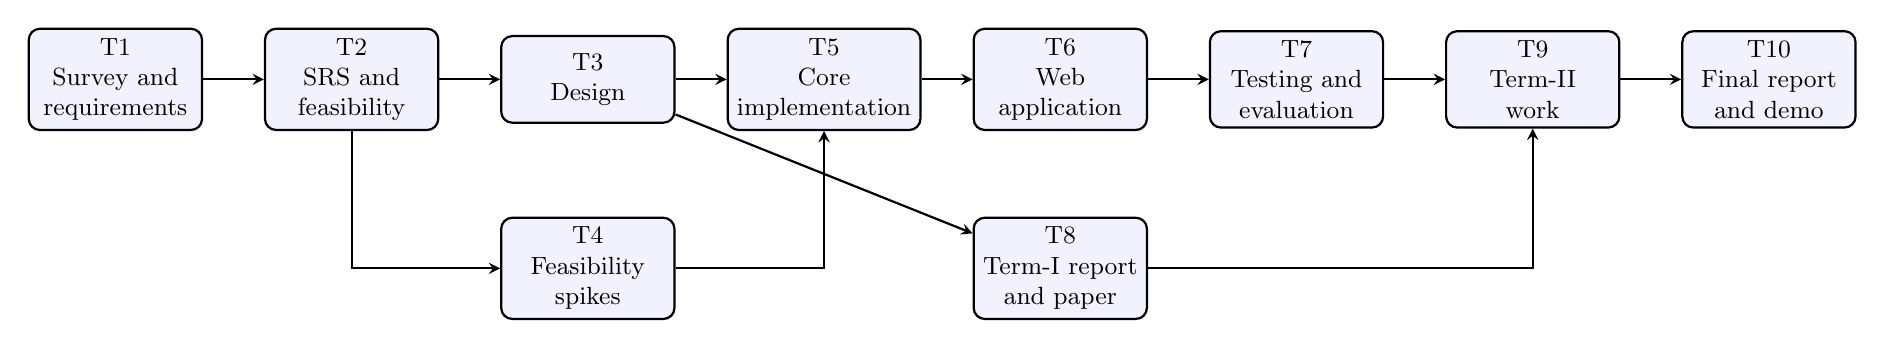
\begin{tikzpicture}[>=stealth, thick,
  task/.style={draw, rounded corners, minimum width=2.2cm, minimum height=1.1cm, align=center, font=\small, fill=blue!5}]
\node[task] (t1) at (0,0) {T1\\Survey and\\requirements};
\node[task] (t2) at (3,0) {T2\\SRS and\\feasibility};
\node[task] (t3) at (6,0) {T3\\Design};
\node[task] (t4) at (6,-2.4) {T4\\Feasibility\\spikes};
\node[task] (t5) at (9,0) {T5\\Core\\implementation};
\node[task] (t6) at (12,0) {T6\\Web\\application};
\node[task] (t7) at (15,0) {T7\\Testing and\\evaluation};
\node[task] (t8) at (12,-2.4) {T8\\Term-I report\\and paper};
\node[task] (t9) at (18,0) {T9\\Term-II\\work};
\node[task] (t10) at (21,0) {T10\\Final report\\and demo};
\draw[->] (t1) -- (t2);
\draw[->] (t2) -- (t3);
\draw[->] (t2) |- (t4);
\draw[->] (t3) -- (t5);
\draw[->] (t4) -| (t5);
\draw[->] (t5) -- (t6);
\draw[->] (t6) -- (t7);
\draw[->] (t3) -- (t8);
\draw[->] (t7) -- (t9);
\draw[->] (t8) -| (t9);
\draw[->] (t9) -- (t10);
\end{tikzpicture}}
\caption{Task network}
\label{fig:tasknet}
\end{figure}

\subsection{Timeline Chart}
A project timeline chart for the entire project is presented in the project planner. Please refer Annexure~\ref{app:plan} for the planner and the timeline chart (Figure~\ref{fig:gantt}).


\section{Team Organization}
\label{sec:team}
The team consists of four students supervised by the internal guide. Work is divided by subsystem, and each subsystem has one owner and one reviewer.
\subsection{Team structure}
Table~\ref{tab:roles} lists the roles. The assignment of members to roles is to be completed by the team.

\begin{table}[!htbp]
\begin{center}
\def\arraystretch{1.4}
\begin{tabularx}{\textwidth}{| p{4.2cm} | X | p{2.8cm} |}
\hline
Role & Responsibilities & Member \\ \hline
Agent and verification & Planner, parallel search, synthesis prompt, claim verification, action store, evaluation harness & [to be filled] \\ \hline
Connectors and model router & Composio, MCP, Firecrawl and sample connectors; free-tier router, cooldowns and cache & [to be filled] \\ \hline
Memory service & FastAPI service, SQLite ledger, Oracle Agent Memory adapter, memory policy & [to be filled] \\ \hline
Web application and testing & Ask, Brief, Memory and Connections screens; event stream client; tests and documentation & [to be filled] \\ \hline
Internal guide & Review of design and progress, approval of milestones & Prof. [Guide Name] \\ \hline
\end{tabularx}
\end{center}
\caption{Team roles}
\label{tab:roles}
\end{table}

\subsection{Management reporting and communication}
Progress is reported to the internal guide in the project slots of the laboratory time table and recorded in the assessment sheet. Within the team, work is tracked in the shared Git repository: each change is a commit with a descriptive message, design decisions are recorded in the project documentation, and the automated tests and the evaluation are run before a change is merged.

